\section{Processi organizzativi}
\subsection{Gestione dei processi}
\subsubsection{Attività}
\paragraph{Gestione delle comunicazioni}
\subparagraph{Comunicazione interna}
Viene utilizzato un gruppo Telegram\G\ per comunicare informalmente fra i membri del \textit{team}.
Il servizio fornisce il vantaggio di essere un'applicazione 
multipiattaforma\G\ e disponibile nelle versioni \textit{desktop}, \textit{web} e \textit{mobile}. Inoltre è possibile catalogare e tenere traccia degli argomenti tramite l'uso di \textit{hashtag}\G\ (per esempio: \#analisiRequisiti), e chiamare all'attenzione un dato membro attraverso l'utilizzo del comando chiocciola (per esempio: @GordonFreeman).

\subparagraph{Comunicazione esterna}
Il \textit{Responsabile di Progetto} è la persona preposta a mantenere i contatti con 
individui esterni al gruppo. Per tali comunicazioni è stato creato il 
seguente indirizzo di posta elettronica:
\begin{center}
	starklabs.swe@gmail.com
\end{center}
Tutti i componenti del gruppo possono accedere all'indirizzo di posta, tuttavia solo 
il \textit{Responsabile di Progetto} può inviare comunicazioni con tale indirizzo email. 
Tutte le email ricevute verranno automaticamente inoltrate agli indirizzi personali dei membri del \textit{team}.

\subparagraph{Composizione email}
\begin{itemize}
\item \textbf{Destinatario:}
\begin{itemize}
\item I destinatari possono essere il Proponente (Giulio Paci e l'azienda MIVOQ s.r.l.), il Prof. Tullio Vardanega e il Prof. Riccardo Cardin.
\end{itemize}
\item \textbf{Mittente:}
\begin{itemize}
\item L'unico indirizzo utilizzabile è starklabs.swe@gmail.com e può essere usato solamente dal \textit{Responsabile di Progetto}.
\end{itemize}

\item \textbf{Oggetto:} l'oggetto deve contenere la dicitura [UNIPD-TTS] così come è stato specificato nel capitolato dell'azienda Proponente. Nel caso il messaggio sia una risposta è consigliabile aggiungere la particella “Re:” all'inizio dell'oggetto per rendere chiara la distinzione del livello di risposta; se si dovesse trattare di un inoltro si deve usare la particella “I:”. L'oggetto non va mai cambiato.

\item \textbf{Corpo:} in caso di risposta da parte dell'azienda MIVOQ o del Committente,
risulta utile la citazione della frase a cui si intende rispondere. Il modello per citare correttamente una porzione del messaggio deve rispettare le seguenti regole: devono essere presenti data e ora della mail a cui si risponde, il nome del mittente e il suo 
indirizzo email tra parentesi angolari. Per esempio: <starklabs.swe@gmail.com>, 
la dicitura “ha scritto:” e infine il testo con all'inizio una parentesi angolare chiusa (“>testo di prova”). 
Se dovessero essere presenti alcune parti con uno o 
più destinatari specifici, il nome dovrà essere indicato all'inizio del paragrafo attraverso la dicitura: \textit{@destinatario}.

\item \textbf{Allegati:} qualora vi fosse necessità, è possibile allegare alcuni \textit{file} al 
messaggio email. Possono per esempio essere allegati i verbali di eventuali incontri con 
Proponente o Committente, oppure \textit{file} facenti parte della documentazione spiegata in sezione \hyperref[sec:suddivisioneDocumenti]{3.1.4.5 Suddivisione dei documenti}.
\end{itemize}


\paragraph{Gestione delle riunioni}
\subparagraph{Riunioni interne}
\begin{itemize}
\item \textbf{Frequenza:} le riunioni del gruppo di lavoro avranno cadenza settimanale; 

\item \textbf{Convocazione:} Il \textit{Responsabile di Progetto} ha il compito di convocare le riunioni generali, a 
cui dovranno partecipare tutti i membri del gruppo.
Su decisione del \textit{Responsabile di Progetto} le riunioni possono coinvolgere anche 
solo specifici componenti del gruppo, a seconda del ruolo che si ritiene più 
utile in una data fase del progetto. Al termine di ogni riunione viene redatto 
un verbale.
Il \textit{Responsabile} deve convocare l'assemblea con almeno un giorno di preavviso
attraverso l'invio di una comunicazione ufficiale nel gruppo Telegram\G, messa in rilievo tramite l'uso dell'\textit{hashtag}\G\ \#riunioneDATA, 
con DATA espressa nel formato d/mmmm/yyyy. Per esempio: \#riunione8marzo2016 raccoglie i messaggi inerenti alla riunione tenutasi in data 8 marzo 2016. Nel corpo del messaggio deve essere specificato:
\begin{itemize}
	\item \textbf{Data}: data e ora prevista;
	\item \textbf{Luogo}: luogo previsto;
	\item \textbf{Tipo}: ordinaria o straordinaria;
	\item \textbf{Ordine del giorno}: elenco ordinato delle voci da esaminare.
\end{itemize}

Ogni componente del gruppo deve rispondere al messaggio nel più breve tempo possibile, confermando la presenza o giustificando l'eventuale assenza. In assenza di una risposta di uno o più membri entro 24 ore, il \textit{Responsabile di Progetto} ha il compito di contattare telefonicamente gli interessati. Una volta ricevute le 
risposte e verificata l'assenza o presenza dei membri convocati, il 
\textit{Responsabile di Progetto} ha la possibilità di decidere se confermare o 
posticipare la riunione, in modo da permettere la presenza di tutti i membri chiamati; 
tutte le eventuali modifiche dovranno essere notificate tramite lo stesso \textit{hashtag} utilizzato per organizzare la riunione. 

\item \textbf{Verbale:} il verbale di riunione interna si presenta in forma di documento 
informale, utile al solo scopo di fissare in modo ordinato i punti principali trattati e le relative soluzioni proposte. Il verbale deve essere redatto come documento testuale utilizzando la funzione \textit{Notebooks}\G\ di Teamwork\G. In questo modo si facilita la condivisione, tra tutti i membri del gruppo, di un documento mantenuto aggiornato dal segretario della riunione. Tale ruolo viene scelto a rotazione tra i membri convocati. È inoltre compito del segretario annotare ogni argomento trattato e controllare che venga rispettato l'ordine del giorno.

\end{itemize}

\subparagraph{Riunioni esterne}
\begin{itemize}
\item \textbf{Convocazione}: in questo caso viene utilizzata l'email starklabs.swe@gmail.com attraverso la quale il \textit{Responsabile di Progetto} si occupa di contattare l'azienda Proponente e di mettere in cc\G\ i membri del gruppo. Per quanto sia auspicabile una riunione plenaria, eventuali assenze 
dei componenti del \textit{team} non causeranno posticipazioni o spostamenti delle 
date di incontro, dovendo ovviamente considerare gli impegni dell'azienda stessa.

\item \textbf{Verbale}: in caso di riunione con il Committente o il Proponente, il verbale è un 
documento che assume carattere ufficiale e che pertanto viene redatto secondo uno schema 
specifico.
Per agevolare la scrittura di tale documento viene utilizzato un \textit{template}\G\ 
\LaTeX\ per definire la struttura e organizzare i contenuti. Tale documento 
dovrà essere redatto e inviato come allegato in risposta all'email di convocazione 
dell'assemblea al Proponente Giulio Paci direttamente dal segretario scelto tra i membri presenti. 
\end{itemize}


\paragraph{Gestione del sistema dei task} Il sistema selezionato per la gestione dei \textit{task}\G\ è Teamwork\G, un servizio \textit{web} di \textit{project management}\G. Le viste presenti sono:
\begin{itemize}
\item \textbf{Dashboard}: dove vengono visualizzati i progetti attivi e le ultime notizie relative ad essi;

\item \textbf{Everything}: che consente di visualizzare i \textit{task}, le \textit{milestone}\G\ e i \textit{file} con possibilità di filtrarli per data;

\item \textbf{Project}: permette di visualizzare la lista di tutti i progetti suddivisi per categoria e ne consente l'accesso;

\item \textbf{Calendar}: mostra un calendario per la gestione degli impegni e delle scadenze;

\item \textbf{Statuses}: consente di verificare gli stati dei collaboratori del progetto;

\item \textbf{People}: permette di visualizzare l'elenco dei singoli elementi del gruppo di lavoro e di accedere al loro profilo.    
\end{itemize}

Le funzionalità principali si hanno in seguito all'accesso al progetto desiderato. Esse si suddividono nei seguenti punti:
\begin{itemize}
\item Aggiunta di nuovi \textit{task}, ed eventualmente di sotto \textit{task}, da associare ad uno o più membri del \textit{team};

\item Assegnazione a ciascun \textit{task}\ di una data d'inizio e di completamento;

\item Aggiunta di nuove \textit{milestone}\ con relativi dettagli come responsabile, descrizione e data di scadenza;

\item \textit{Upload}\G\ di file potenzialmente utili al gruppo di lavoro;

\item Utilizzo di un blocco note.
 
\end{itemize}

\paragraph{Gestione delle milestone} 
Il \textit{Responsabile di Progetto} ha il compito di pianificare i punti di controllo che il \textit{team} deve raggiungere, assicurandosi che ogni \textit{task}\G\ necessario al suo soddisfacimento venga terminato entro la data prestabilita.

\paragraph{Gestione dei task} 
È compito del \textit{Responsabile di Progetto} individuare ogni singolo \textit{task}\G\ e, al seguito di un'accurata valutazione, assegnarlo al membro del gruppo più adatto. Deve inoltre associare una data di inizio e di scadenza di fattibilità. Tutte queste attività possono essere facilmente accedute attraverso l'interfaccia grafica di Teamwork\G.

\paragraph{Gestione dello svolgimento dei task}
Ogni membro del gruppo di lavoro è tenuto ad accettare il \textit{task}\G\ assegnatogli dal \textit{Responsabile di Progetto} e fare quanto possibile per portarlo a termine entro la data di scadenza. Nel caso in cui l'assegnatario non fosse in grado di adempire al suo compito è tenuto a renderlo noto al \textit{Responsabile di Progetto} entro 24 ore dall'assegnazione del \textit{task}, altrimenti quest'ultimo verrà considerato come accettato; solo dopo un'accurata valutazione delle motivazioni riportate, il \textit{Responsabile di Progetto} può provvedere a trovare un nuovo membro da incaricare allo svolgimento del \textit{task}.

\subsubsection{Procedure}
\paragraph{Generazione di una milestone}
Dopo aver avuto accesso al progetto di Teamwork\G, il \textit{Responsabile di Progetto} deve eseguire i seguenti passi per generare una \textit{milestone}\G:
\begin{itemize}
\item [1.] Cliccare sul pulsante \textit{"Add a milestone"};
\item [2.] Definire il titolo della \textit{milestone};
\item [3.] Definire la data di scadenza;
\item [4.] Assegnarla ad un responsabile.
\end{itemize}

\paragraph{Assegnazione di un task}
Dopo essere acceduto al progetto di Teamwork\G, il \textit{Responsabile di Progetto} deve eseguire i seguenti passi, mostrati anche in \hyperref[sec:Figura6]{Figura 6}, per generare un \textit{task}\G\:
\begin{itemize}
\item [1.] Cliccare sul pulsante \textit{"Add a task"};
\item [2.] Definire il titolo del \textit{task};
\item [3.] Definire la data di inizio;
\item [4.] Definire la data di scadenza;
\item [5.] Assegnarlo ad uno o più membri del gruppo.
\end{itemize}

\begin{figure}[htbp]
\centering
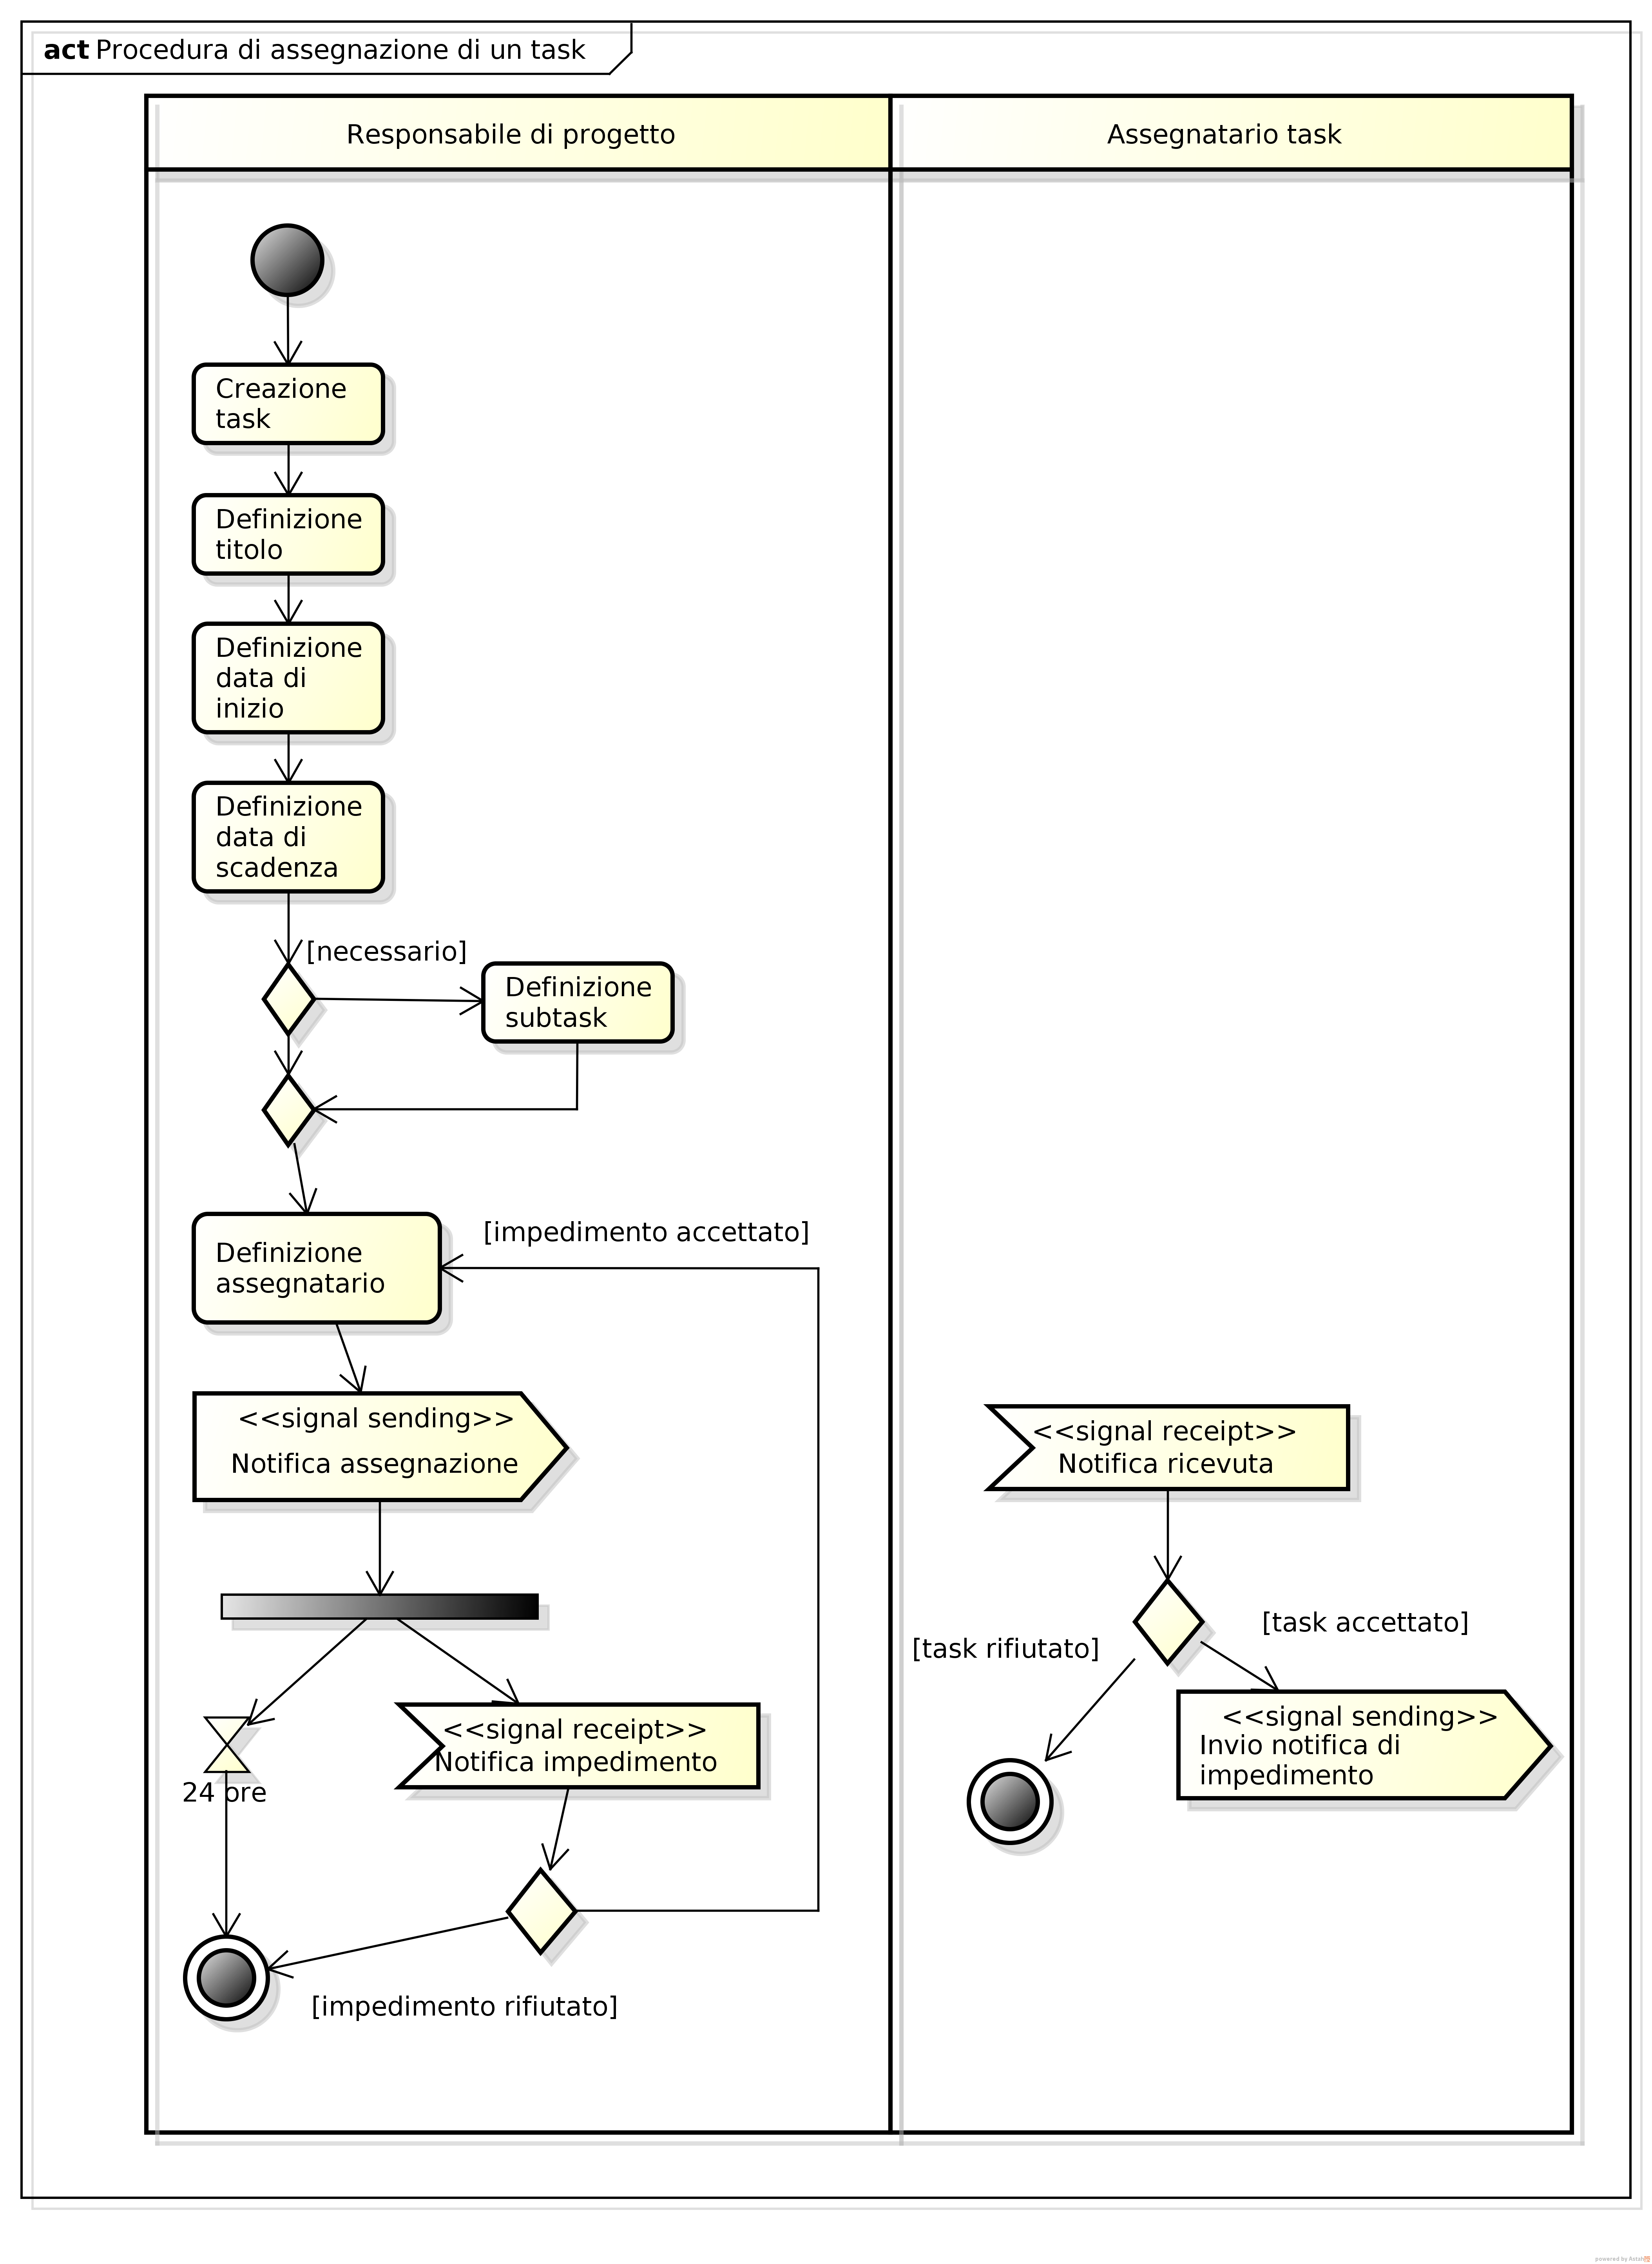
\includegraphics[scale=0.5]{immagini/procedura_di_assegnazione_di_un_task.png}
\captionsetup{labelfont=bf}
\caption{Diagramma di attività - Procedura di assegnazione di un task}\label{sec:Figura6}
\end{figure}

\paragraph{Svolgimento di un task}
Il membro assegnatario del \textit{task}\G, ricevuta la notifica e non avendo alcun impedimento, deve procedere secondo le seguenti direttive, mostrate anche in \hyperref[sec:Figura7]{Figura 7}:
\begin{itemize}
\item [1.] Se il \textit{task} ricevuto ha una scadenza più immediata rispetto a quello su cui sta lavorando, deve sospendere lo svolgimento di quest'ultimo, metterlo in coda e dedicarsi al \textit{task} appena notificato;
\item [2.] Se, dopo aver iniziato lo svolgimento del \textit{task}, si riceve la notifica di uno nuovo con scadenza più immediata si procede come riportato nel punto precedente;
\item [3.] Se si dovesse superare la data di scadenza prevista, è necessario impostare il \textit{tag}\G\ "\textit{Delay}" dal sistema offerto su Teamwork\G. Questa situazione si può verificare se:
\begin{itemize}
\item [-] Il tempo assegnato dal \textit{Responsabile di progetto} non è sufficiente al completamento del \textit{task};
\item [-] Il \textit{task} in ritardo sta alle dipendenze di un altro \textit{task} non ancora completato;
\item [-] L'assegnatario è rallentato da cause esterne non rese note al \textit{Responsabile di Progetto};
\item [-] Il membro incaricato non ha a disposizione tutte le conoscenze necessarie per un corretto svolgimento del \textit{task}.
\end{itemize}
Spetta al \textit{Responsabile di Progetto} fare in modo che i primi due casi non si verifichino.

\item [4.] Al completamento del lavoro l'assegnatario deve spuntare il \textit{task} dalla lista presente su Teamwork\G;
\item [5.] A questo punto può proseguire con lo svolgimento dei \textit{task} rimanenti riprendendo la procedura dall'inizio.
\end{itemize}

\begin{figure}[htbp]
\centering
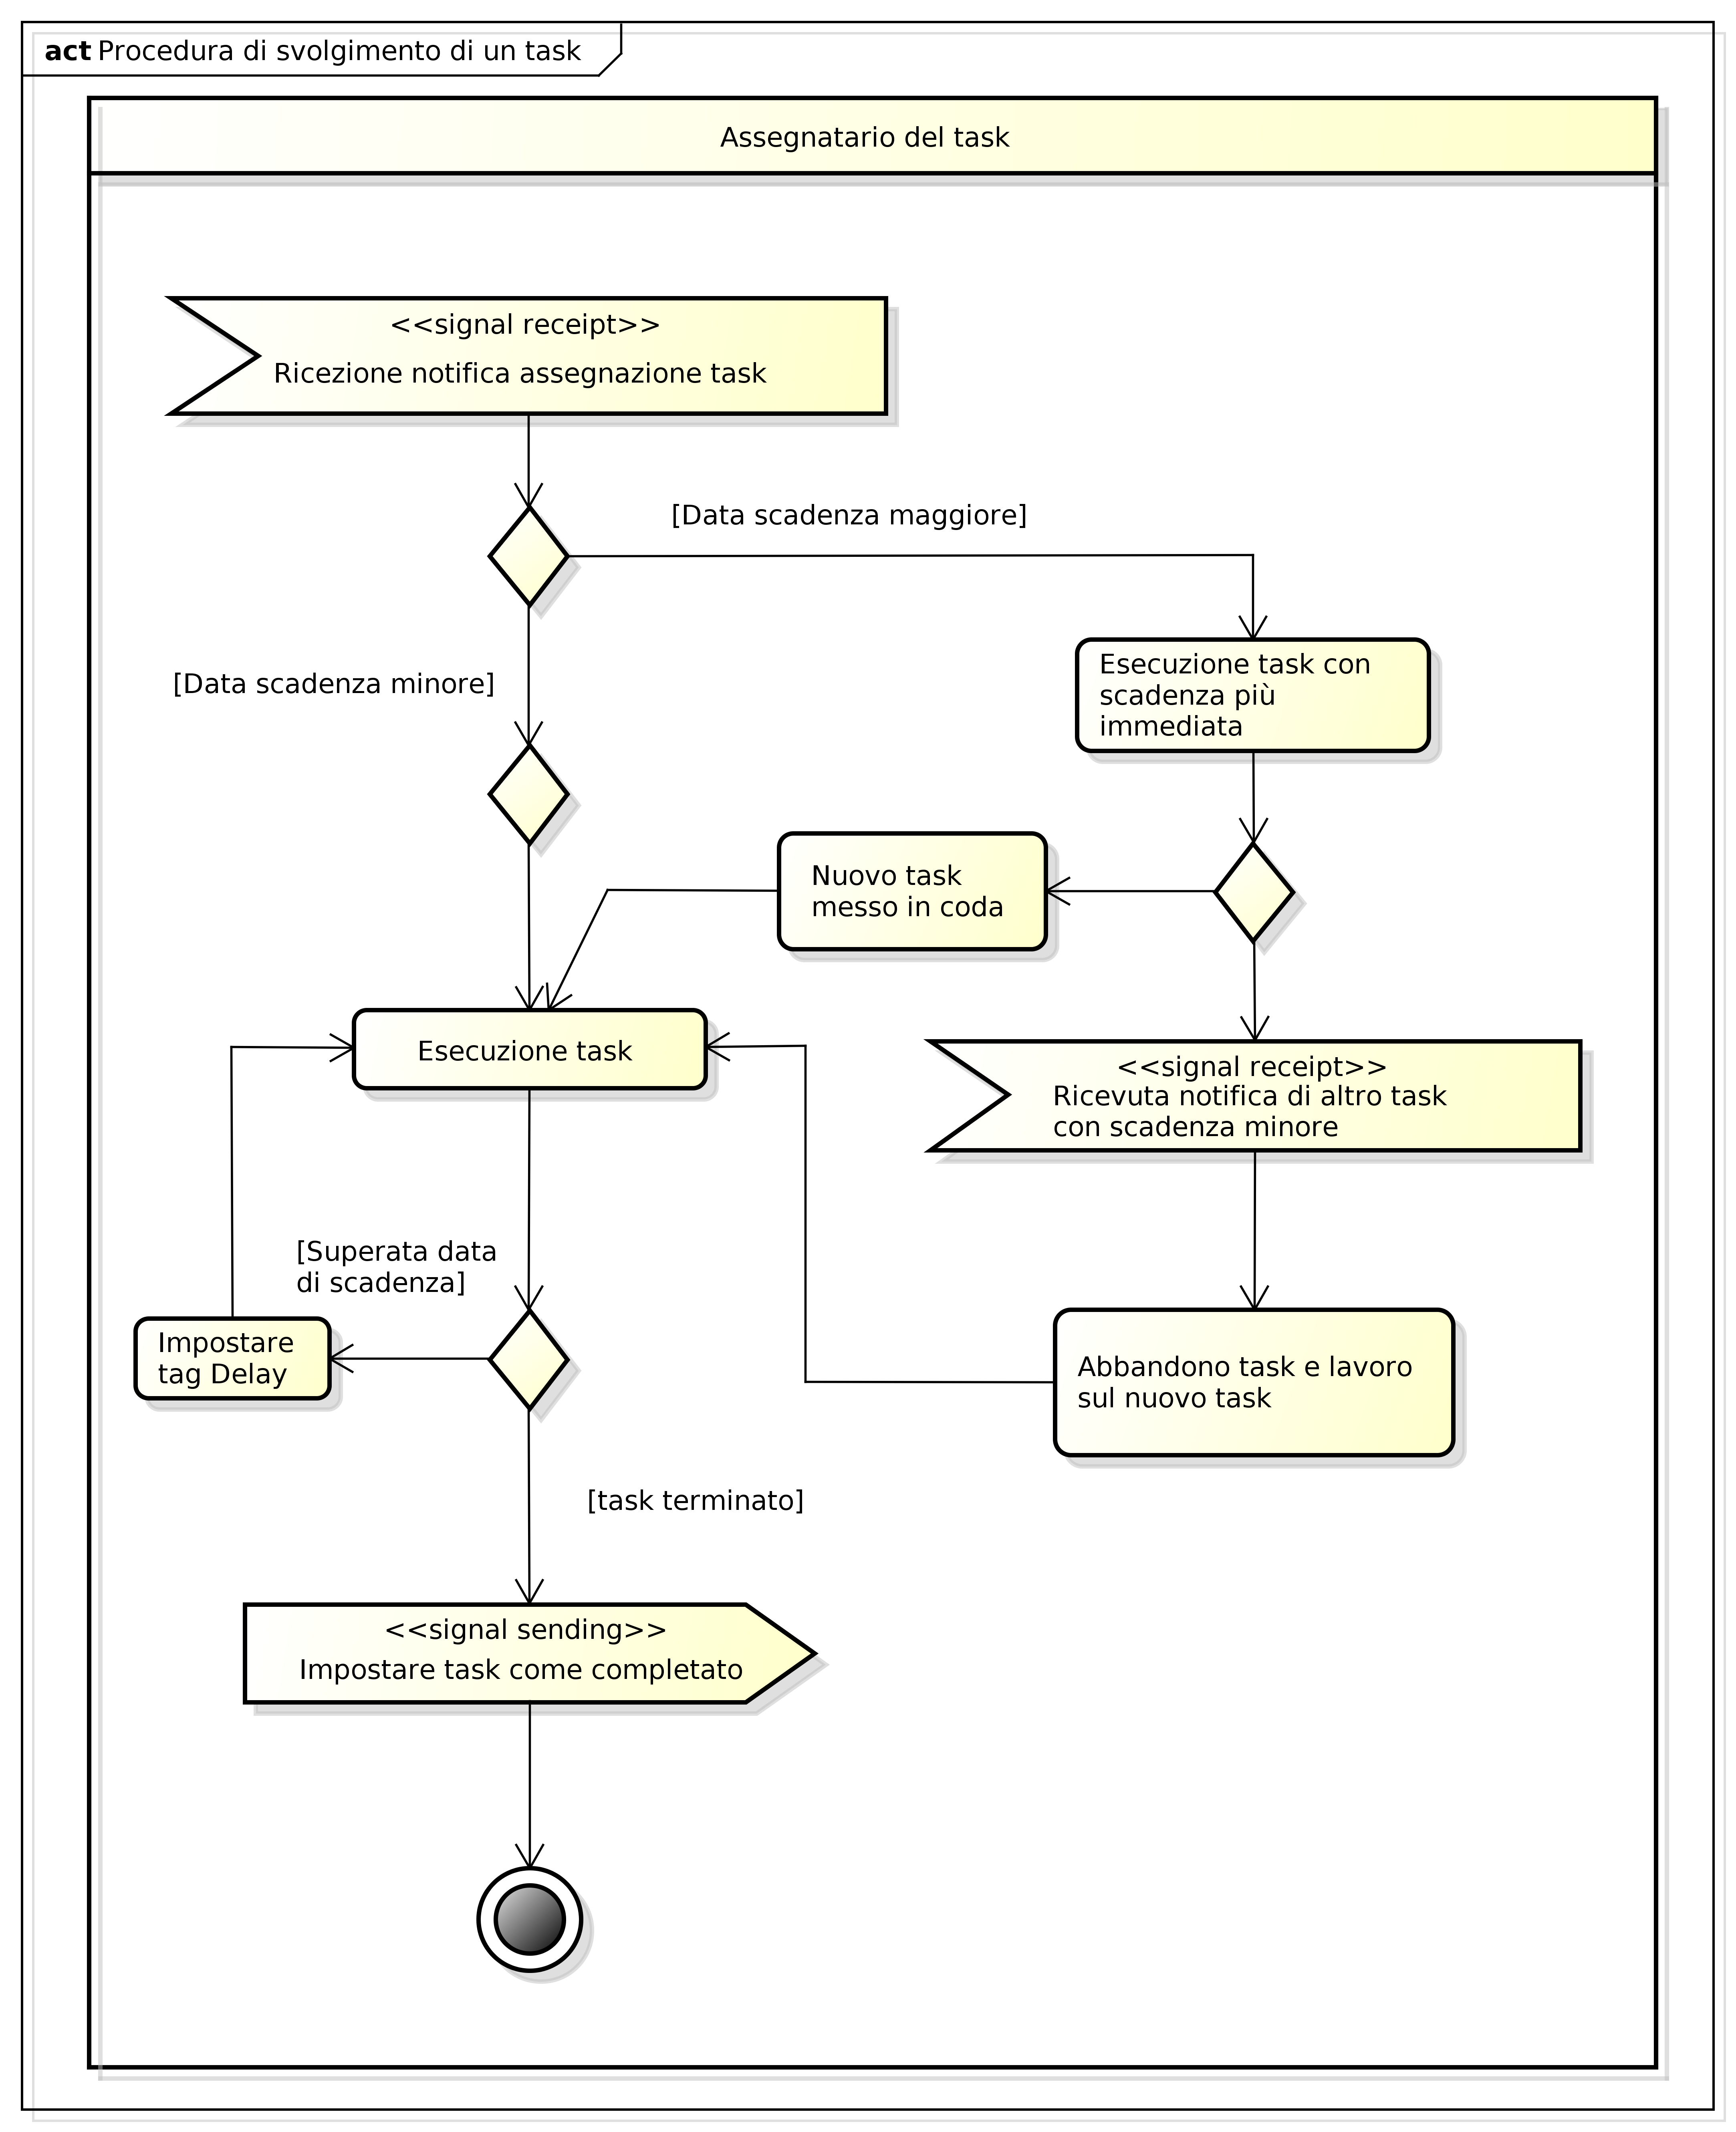
\includegraphics[scale=0.5]{immagini/procedura_di svolgimento_di_un_task.png}
\captionsetup{labelfont=bf}
\caption{Diagramma di attività - Procedura di svolgimento di un task}\label{sec:Figura7}
\end{figure}

\paragraph{Rilevamento dei rischi}
È compito del \textit{Responsabile di Progetto} individuare i rischi trovati nel \textit{Piano di Progetto v1.0.0}. Questa attività necessita di un continuo monitoraggio, in quanto è plausibile che insorgano nuovi rischi in seguito a quelli rilevati nella fase preliminare. In tal caso il \textit{Responsabile di Progetto} deve agire come segue:
\begin{itemize}
\item [1.] Registrare il resoconto effettivo dei rischi nel \textit{Piano di Progetto v1.0.0};
\item [2.] Pianificare per gestire i nuovo rischi;
\item [3.] Aggiornare le metodologie per far fronte alla nuova pianificazione;
\item [4.] Monitorare i nuovo rischi riscontrati durante lo sviluppo del progetto. 
\end{itemize}

\subsubsection{Norme}
\paragraph{Ruoli di Progetto}
Ogni componente del gruppo \GRUPPO\ deve ricoprire almeno una volta ciascuno dei ruoli necessari allo sviluppo del progetto. Nell'assegnazione dei compiti il \textit{team} si impegna a distribuire equamente le ore di lavoro previste per ogni ruolo. Questo criterio ha guidato la stesura del \textit{Piano di Progetto v1.0.0} di cui si rimanda alla lettura.\\
Di seguito vengono presentati i diversi incarichi, delineando per ciascuno mansioni e responsabilità.

\subparagraph{Responsabile di Progetto} Il \textit{Responsabile di Progetto} rappresenta il \textit{team} e il progetto nei confronti di Committente e Proponente; accentra le responsabilità di scelta e approvazione. Detiene inoltre le seguenti responsabilità:
\begin{itemize}
\item Pianificazione e coordinamento delle attività;
\item Gestione e controllo delle risorse;
\item Analisi e gestione dei rischi;
\item Approvazione dei documenti;
\item Assicurarsi che tutte le attività svolte siano conformi alle \textit{Norme di Progetto
v1.0.0} e rispettino la pianificazione effettuata nel \textit{Piano di Progetto v1.0.0}.
\end{itemize}  

\subparagraph{Amministratore di Progetto} L' \textit{Amministratore di Progetto} deve svolgere i seguenti compiti:
\begin{itemize}
\item Assicurarsi che tutte le risorse siano presenti e operanti; 
\item Garantire un'infrastruttura funzionale;
\item Fornire procedure che servono a garantire la qualità del prodotto uscente da un
determinato compito.
\end{itemize}

\subparagraph{Analista} L' \textit{Analista} deve svolgere i seguenti compiti:
\begin{itemize}
\item Tradurre il bisogno del cliente in una specifica utile per trovare una soluzione;
\item Comprendere la complessità del problema;
\item Capire il dominio nel quale lavora il cliente;
\item Analizzare il dominio applicativo e le specifiche per poi produrre i documenti di analisi.
\end{itemize}

\subparagraph{Progettista} Il \textit{Progettista} deve svolgere i seguenti compiti:
\begin{itemize}
\item Individuare la tecnologia più idonea per risolvere il problema indicato dall'\textit{Analista};
\item Descrivere il funzionamento interno del sistema a diversi livelli di dettaglio;
\item Produrre una soluzione comprensibile e attuabile. 
\end{itemize}

\subparagraph{Programmatore} Il \textit{Programmatore} ha responsabilità sulle attività di codifica e pertanto deve svolgere i seguenti compiti:
\begin{itemize}
\item Scrivere codice documentato, versionato e manutenibile;
\item Implementare le soluzioni descritte dal \textit{Progettista};
\item Implementare i \textit{test} sul codice prodotto. 
\end{itemize}

\subparagraph{Verificatore} Il \textit{Verificatore} è il responsabile delle attività di verifica e pertanto deve svolgere i seguenti compiti:
\begin{itemize}
\item Controllare che vengano rispettate le norme di progetto;
\item Assicurarsi la conformità di ogni stadio del ciclo di vita\G\ del prodotto.
\end{itemize}

\subsubsection{Strumenti}

\paragraph{TeXstudio} TeXstudio\G\ è l'\textit{editor} di testo multipiattaforma \textit{open-source}\G\ utilizzato per scrivere documenti in \LaTeX.
\paragraph{Teamwork} Teamwork\G\ è l'applicazione \textit{web} scelta per la gestione dei \textit{task}\G; permette anche di gestire un calendario dove inserire note o fissare appuntamenti e/o traguardi importanti.
\paragraph{Astah} Astah\G\ è l'applicativo scelto per la creazione di grafici UML\G. La versione adottata è quella \textit{Professional}, resa disponibile gratuitamente per un utilizzo da parte di studenti.
\paragraph{Microsoft Project 2016} Microsoft Project 2016 è il \textit{software} utilizzato per la creazione dei grafici di Gantt\G. Si utilizza il contratto Microsoft MSDN-AA (\textit{Academic Alliance}) reso disponibile dal Dipartimento di Matematica dell'Università degli Studi di Padova in accordo con Microsoft.
\paragraph{Telegram} Si utilizza Telegram\G\ per una comunicazione informale all'interno del 
gruppo. Inoltre Telegram fornisce il vantaggio di essere un'applicazione 
multipiattaforma\G\ disponibile nelle seguenti versioni: \textit{desktop}, \textit{web} e \textit{mobile}.
\paragraph{Microsoft Office PowerPoint} PowerPoint\G\ è il software utilizzato per creare presentazioni.

\subsection{Gestione delle infrastrutture}

\paragraph{Attività} 
\subparagraph{Gestione del repository} Il gruppo ha deciso di utilizzare un repository\G\ utile a svolgere funzioni diverse, ma necessarie, allo sviluppo del sistema finale. Una volta iscritto, ciascun membro ha la possibilità di creare il suo \textit{branch}\G\ personale contenente una copia dei file originali del \textit{branch} \textit{master} in modo da poter lavorare su delle copie in locale.

\subparagraph{Gestione del messaggio di commit} Per mantenere l'ambiente di lavoro il meno ambiguo possibile, è stato deciso di adottare un formato standard per andare a scrivere il messaggio della \textit{commit}\G.

\paragraph{Procedure} 
\subparagraph{Installazione di Git} La procedura di installazione varia a seconda del sistema operativo utilizzato. Per i sistemi Linux\G\ occorre rispettare la seguente procedura:
\begin{itemize}
\item Aprire il terminale;
\item Immettere il comando \textit{sudo apt-get update};
\item Immettere il comando \textit{apt-get install git}.
\end{itemize}
Per sistemi OS X\G:
\begin{itemize}
\item Recarsi nella sezione dedicata ai \textit{download} \url{https://git-scm.com/download/mac};
\item Scaricare il \textit{file} in formato DMG\G;
\item Aprire il file appena scaricato;
\item Lanciare l'installazione cliccando su\textit{ git.pkg}.
\end{itemize}
Infine per i sistemi Windows\G, è necessario fare quanto segue:
\begin{itemize}
\item Accedere al sito ufficiale \url{https://git-for-windows.github.io};
\item Scaricare l'eseguibile;
\item Lanciare l'eseguibile;
\item Seguire la procedura riportata dalla finestra di dialogo.
\end{itemize}

\subparagraph{Creazione di una cartella locale di repository} Seguire la seguente procedura:
\begin{itemize}
\item Creare una nuova cartella;
\item Aprire il terminale;
\item Collocarsi all'interno della cartella appena creata;
\item Eseguire il comando \textit{git init}.
\item Immettere il comando \textit{git clone <indirizzo>}, sostituendo <indirizzo> con l'URL del progetto su GitHub\G.
\end{itemize}

\subparagraph{Creazione del branch personale} Per creare il \textit{branch}\G\ personale occorre seguire i seguenti passi:
\begin{itemize}
\item Muoversi nella cartella di \textit{repository}\G.
\item Accedere alla cartella di progetto;
\item Eseguire il comando \textit{git branch <nome>}, sostituendo <nome> con il nome del nuovo \textit{branch} da creare.
\end{itemize}

\subsubsection{Norme}
\paragraph{Repository}
\subparagraph{Nomi dei file in SiVoDiM} I \textit{file} e le cartelle presenti
nel \textit{repository}\G\ devono essere conformi al seguente formalismo tratto dallo Standard
ISO\G\ 9660:1999 (Level 2):
\begin{itemize}
\item I caratteri usati sono solo quelli minuscoli a-z, 0-9, l’\textit{underscore}\G\ e il punto (esempio: nome\_del\_documento.tex);
\item Non sono ammessi caratteri accentati;
\item I nomi non possono includere spazi o finire con un punto (.);
\item I nomi non devono contenere più di un punto (.) utilizzato per separare il nome del \textit{file} dall'estensione (esempio: studio\_di\_fattibilita\_v1\_0\_0.pdf);
\item I nomi non devono essere più lunghi di 21 caratteri esclusi i 3 destinati all’estensione.
\end{itemize}

\subparagraph{Struttura di SiVoDiM}  Le cartelle nel repository\G\ verranno organizzate nel seguente modo a partire dalla \textit{root}\G:
\begin{itemize}
\item \textbf{Documenti}: in essa sono presenti le seguenti cartelle corrispondenti alle varie fasi del processo di sviluppo:
\begin{itemize}
\item \textbf{RR}: contenente i documenti e i file necessari alla revisione dei requisiti;
\item \textbf{RP}: contenente i documenti e i file necessari alla revisione di progettazione;
\item \textbf{RQ}: contenente i documenti e i file necessari alla revisione di qualifica;
\item \textbf{RA}: contenente i documenti e i file necessari alla revisione dei accettazione;
\end{itemize}
\item \textbf{Codice}: la struttura di questa cartella verrà fornita in una fase successiva del lavoro.
\end{itemize}

\subparagraph{Messaggio di commit} Il messaggio di commit\G\ dovrà
essere conforme alla seguente notazione:
\begin{center}
Desc:\\
Data:\\
Note:\\
\end{center}
dove:
\begin{itemize}
\item \textbf{Desc}: fornisce una descrizione esaustiva dell’attività svolta;
\item \textbf{Data}: fornisce la data in cui si è apportata la modifica;
\item \textbf{Note}: aiuta a specificare lo stato del lavoro, nello specifico si adotteranno le seguenti notazioni:
\begin{itemize}
\item [-]{C} se il lavoro è stato completato;
\item [-]{NC} se il lavoro non è stato completato;
\item [-]{V} se il lavoro necessita de verifica;
\end{itemize}
\end{itemize}

\subsubsection{Strumenti}
\paragraph{Git} Git\G\ è il sistema di controllo di versione utilizzato per il \textit{repository}\G\ del \textit{team}.

\paragraph{GitHub} GitHub\G\ è il servizio \textit{web} di \textit{hosting}\G\ adottato per tenere una
copia del \textit{repository}\G\ del progetto.

\paragraph{Dropbox} Dropbox\G\ è lo strumento di \textit{cloud}\G\ che si è scelto
per gestire \textit{file} che non necessitano di essere sottoposti a controllo di versione.

\paragraph{Sistema Operativo} I membri del gruppo operano su tre diversi sistemi operativi:
\begin{itemize}
\item Ubuntu 14.04\G;
\item Linux Mint 17\G;
\item Windows 10\G;
\item OS X 10.11\G.
\end{itemize} 

\subsection{Formazione dei membri del gruppo}
I membri del gruppo che non hanno conoscenze sufficienti per far fronte ai problemi assegnati dal \textit{Responsabile di Progetto}, dovranno
documentarsi e colmare eventuali lacune durante ore esterne a quelle di lavoro, non imputabili perciò ai costi del Committente.

